\begin{table}[hbtp]
\centering
\newcommand{\LEDsingHeight}{0.55cm}
\caption{Význam stavů svítivé diody na serveru}
\label{tab:serverLED}
\label{tab:LED_man}
\begin{tabular}{|c|c|}
\hline
\textbf{Stav svítivé diody}                                            & \textbf{Význam}                  \\ \hline

\includegraphics[height=\LEDsingHeight/2]{img/manual/black.png}             & server je vypnutý/nemá napájení  \\ \hline

\includegraphics[height=\LEDsingHeight]{img/manual/blue.png}              & server je připraven              \\ \hline

\includegraphics[height=\LEDsingHeight]{img/manual/violet_blink.png} 3x   & nový klient připojen             \\ \hline

\includegraphics[height=\LEDsingHeight]{img/manual/orange_blink.png}   3x & klient se odpojil/byl odpojen    \\ \hline
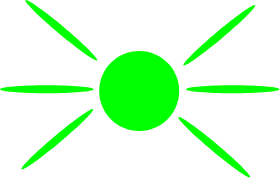
\includegraphics[height=\LEDsingHeight]{img/manual/green.png}             & aktuálně běží hra                \\ \hline

\includegraphics[height=\LEDsingHeight]{img/manual/green_blink.png}       & hra ukončena (výhra/remíza)      \\ \hline
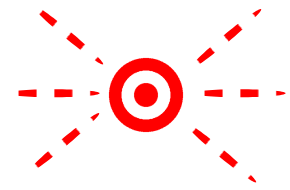
\includegraphics[height=\LEDsingHeight]{img/manual/red_blink.png} 3x      & chyba (nedostatek hráčů pro hru) \\ \hline
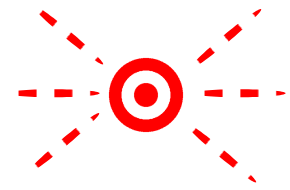
\includegraphics[height=\LEDsingHeight]{img/manual/red_blink.png} stále   & chyba sítě (připojení kabelu)    \\ \hline
\end{tabular}
\end{table}
